\chapter{Single molecule FRET spectroscopy
\label{chpt:smFRET}}

\section{A brief history of FRET
\label{sec:smFRET}}

\textit{The History of FRET: From Conception Through the Labors of Birth}, by Robert M. Clegg~\cite{clegg_history}, is an essential read for those interested in physical chemistry and biophysics. 
The following historical introduction is primarily based on this work, and I would like to give proper attribution to Clegg for this wonderfully thorough read.

The first real reference to \ac{FRET} was presented in 1922 by Franck. 
\enquote{Franck's Principle} presented the theory of fluorescence quenching which was understood to involve \enquote{energy resonance} between two atoms.
The first experiment to indicate the presence of energy transfer at a distance, was performed by Cario and Franck in 1922~\cite{clegg_history}. 
In this experiment a mixture of thallium and mercury vapors were irradiated at 253.6 nm, the wavelength at which mercury, but not thallium, can be excited.
Franck and Cario observed a fluorescent signal arising from the thallium vapor.
They termed this energy transfer \enquote{sensitized fluorescence}~\cite{clegg_history}.

Soon after, in 1928 Kallmann and London presented a quantum mechanical treatment of energy transfer that expanded on the classical definition of \enquote{spectroscopic} cross-sections~\cite{Kallmann_London}.
This work was particularly interesting, as it was the basis for the idea that dipole-dipole interactions could effectively extend the radius of interactions between atoms, namely that physical collision between atoms was not required for energy transfer to occur.
Kallmann and London's derivations gave the correct distance dependence in the case of partial resonance~\cite{clegg_history}. 

\begin{wrapfigure}{r}{0.5\textwidth}
    \centering
    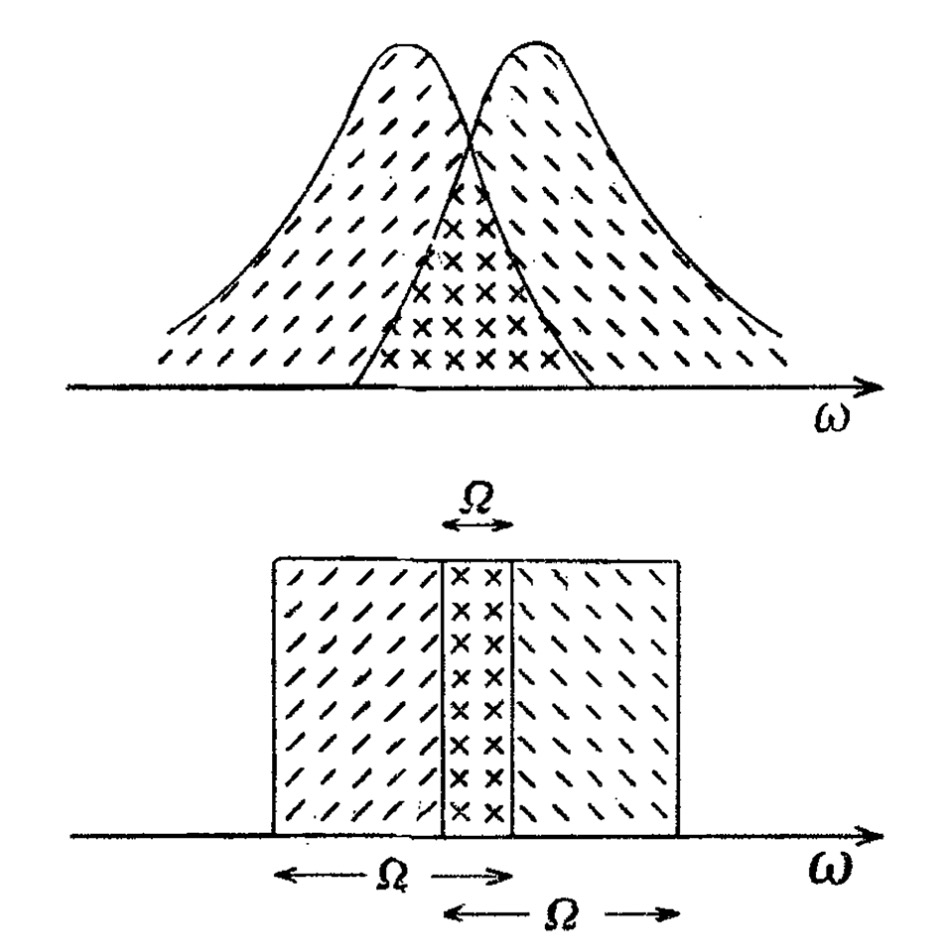
\includegraphics[width=0.48\textwidth]{chapters/figures/spectral_overlap.jpg}
    \caption{\label{fig:spectral_overlap}
    Top: Actual intensity distribution of broadened absorption and emission spectra for a donor and acceptor molecule.
    Bottom: Schematic of absorption and fluorescence spectra to be two rectangles with a width $\Omega$, with overlap of width $\Omega'$.
    Forward slash hatching indicates emission and backward slash hatching indicates absorption.
    Referenced from the English translation of F{\"o}rster's original work~\cite{forster_1948,forster_english_1948}.
    }
\end{wrapfigure}

In 1929 Francis Perrin, son of Jean Baptiste Perrin who contributed to our classical understanding of FRET, expanded the quantum mechanical understanding to solution-based mixtures of fluorescent dyes. 
F. Perrin's work accounted for spectral overlap, however it overestimated transfer efficiency and distance dependence by requiring exact resonance~\cite{clegg_history, forster_1948}.

In 1948 the German physical chemist, Theodor F{"o}rster,
presented the theoretical framework for FRET that we use today. 
In the original paper published in German, F{"o}rster considers the broadening of the absorption and emission spectra, which was necessary for precise calculation of the rate between two quantum states, as discovered by Dirac in 1927~\cite{clegg_history}.
Thus, F{\"o}rster addressed the shortcomings of Perrin's work~\cite{forster_1948} where spectral overlap was attributed mostly to collisions, and instead adequately took into account the distribution of oscillator frequencies in acceptor and donor molecules. 
The diagram in figure~\ref{fig:spectral_overlap} from F{\"o}rster's publication shows the overlap of fluorescence and absorbance spectra for two molecules.
He correctly took into account the overlapping oscillation frequencies of the donors in the excited state and the acceptor molecules in the ground state.
In addition, F{\"o}rster maintained that energy transfer was only possible when the emission of a photon from an excited state of a donor molecule was absorbed by an unexcited neighboring molecule~\cite{forster_1948, forster_english_1948}. 

In his 1946 publication, F{\"o}rster points out that a classical treatment of energy transfer is enough to derive the correct distance relationship for $R_o$. 
However, in subsequent publications he presented a full quantum mechanical treatment~\cite{clegg_history}. 
In doing so, he explicitly defined the overlap integral which described the rate of transfer from an excited donor molecule to an acceptor molecule in its ground state. 
This was done with experimentally derivable quantities i.e., the refraction index, the quantum yield of the acceptor, and the lifetime of the donor. 
He also considered the effects of anisotropy and presented an expression for the the orientation factor, $\kappa^2$. 
Finally, he showed that $R_o$ could be calculated from the overlap integral. 
Thus, F{\"o}rster established an experimentally accessible definition of FRET, the importance of which cannot be understated. 

As F{\"o}rster's work was pivotal in the field, it is not surprising that Fluorescence Resonance Energy Transfer was commonly referred to as F{\"o}rster Resonance Energy Transfer. 
Nonetheless, we must consider the historical context of that era. 
At the time, authorities forcibly removed non-\enquote{Aryan} scientists and political dissenters from their positions, resulting in a dark period for scientific advancement.

Meanwhile, in 1933, F{\"o}rster joined the Nazi Party and the \footnotemark{SA}.
His privileged status allowed him to fill the void left in the field of physical chemistry, and granted him scientific freedom that many of his contemporaries were denied. 
In light of F{\"o}rster's early association with the Nazi Party, many scientists appropriately refrain from using his name in the FRET acronym.

\footnotetext{Sturmabteilung, or \enquote{Storm Troopers}. 
Colloquially called the \enquote{Brownshirts} for their infamous uniform.
The SA was the original paramilitary unit of the Nazi Party, and was responsible for protecting Nazi rallies and disrupting assemblies of opposing parties, among other things.}

\newpage

In discussions with colleagues, the argument has been raised that F{\"o}rster may have capitulated to the racist ideologies of his time, given the immense pressure to do so. 
While I understand the importance of considering historical context, it is evident that F{\"o}rster was a highly intelligent and forward-thinking scientist. Although I cannot presume to know what his personal philosophies were,
I also cannot overlook the fact that he made the decision to join the Nazi party \textit{and} the SA in 1933, years before the war broke out.
His involvement in both groups was a clear endorsement of Hitler's eugenicist mission.

The following quotation by Martin Niem{\"o}ller serves as a powerful reminder of the consequences of remaining passive in the face of atrocity~\cite{martin_niemoller}. 

\begin{quote}
\centering 
\textit{First they came for the socialists, and I did not speak out — because I was not a socialist.}

\textit{Then they came for the trade unionists, and I did not speak out — because I was not a trade unionist.}

\textit{Then they came for the Jews, and I did not speak out — because I was not a Jew.}

\textit{Then they came for me — and there was no one left to speak for me.}
\end{quote}

As a Jewish scientist and second-generation survivor of the Holocaust, I cannot ignore F{\"o}rster's early involvement in the advancement of Nazism.
While it is speculative to suggest that history may have unfolded differently if more prominent thinkers had spoken out against such ideas, the fact remains that F{\"o}rster was not passive. 
On the contrary, he actively aligned himself with the Nazis, and was therefore a Nazi himself. 

To avoid honoring this disturbing history, I choose to refer to FRET as \enquote{Fluorescence} Resonance Energy Transfer. 
My hope is that by sharing this information, others will cease to attribute the \enquote{F} in FRET to \enquote{F{\"o}rster}.
 
\section{Applications of FRET
\label{sec:FRET_applications}}

FRET is an extremely useful technique for studying biochemical interactions on the order of 3 - 10 nm (Fig.~\ref{fig:FRET_concept}C) and is often aptly referred to as a \enquote{spectroscopic ruler}~\cite{stryer_PNAS_1967}. 
Common applications are inter- and intra-molecular interactions, such as protein - protein interactions or conformational changes within macromolecules. 
The basic premise of FRET experiments relies on the attachment of a FRET pair i.e., a pair of spectrally matched donor and acceptor fluorophores.
Commonly used FRET pairs are red and green fluorescent dyes or red and green fluorescent proteins. 
Notably, other color pairs can be used, however for practical reasons red and green are the most common.

FRET experiments are microscopic or spectroscopic in nature.
Optical FRET microscopy requires that molecules are fixed to the surface.
There are many such techniques, including \ac{TIRF}, \ac{STED}, \ac{SMLM}, and \ac{FLIM}. 
These methods are ideal for studying molecules continuously where measurement times are limited by the photobleaching attributes of the fluorophores.  
Thus, surface immobilization is ideal for studying slow conformational dynamics on the order of $0.1 - 10 s$~\cite{lerner_Science_2018}.

One drawback of surface immobilization methods is that they can restrict the movement of molecules, which may interfere with their function. 
In the case of biomolecules, limiting their degrees of freedom can hinder their normal activity. 
Additionally, chemical linkers used to immobilize molecules to the surface may also interact with the molecules and potentially alter their structure or function. 

In FRET spectroscopy experiments, such as \ac{smFRET} and FRET-based \ac{FCS} or \ac{FCCS}, molecules are not immobilized and instead are allowed to freely diffuse.
This eliminates surface related constraints and allows measurement of biomolecules as they move unrestricted through solution, making FRET spectroscopy ideal for studying faster conformational dynamics on the order of $10~\mu s - 0.1~s$~\cite{lerner_Science_2018}. 


\section{Theory of FRET
\label{sec:FRET_theory}}

\begin{figure}
    \centering
    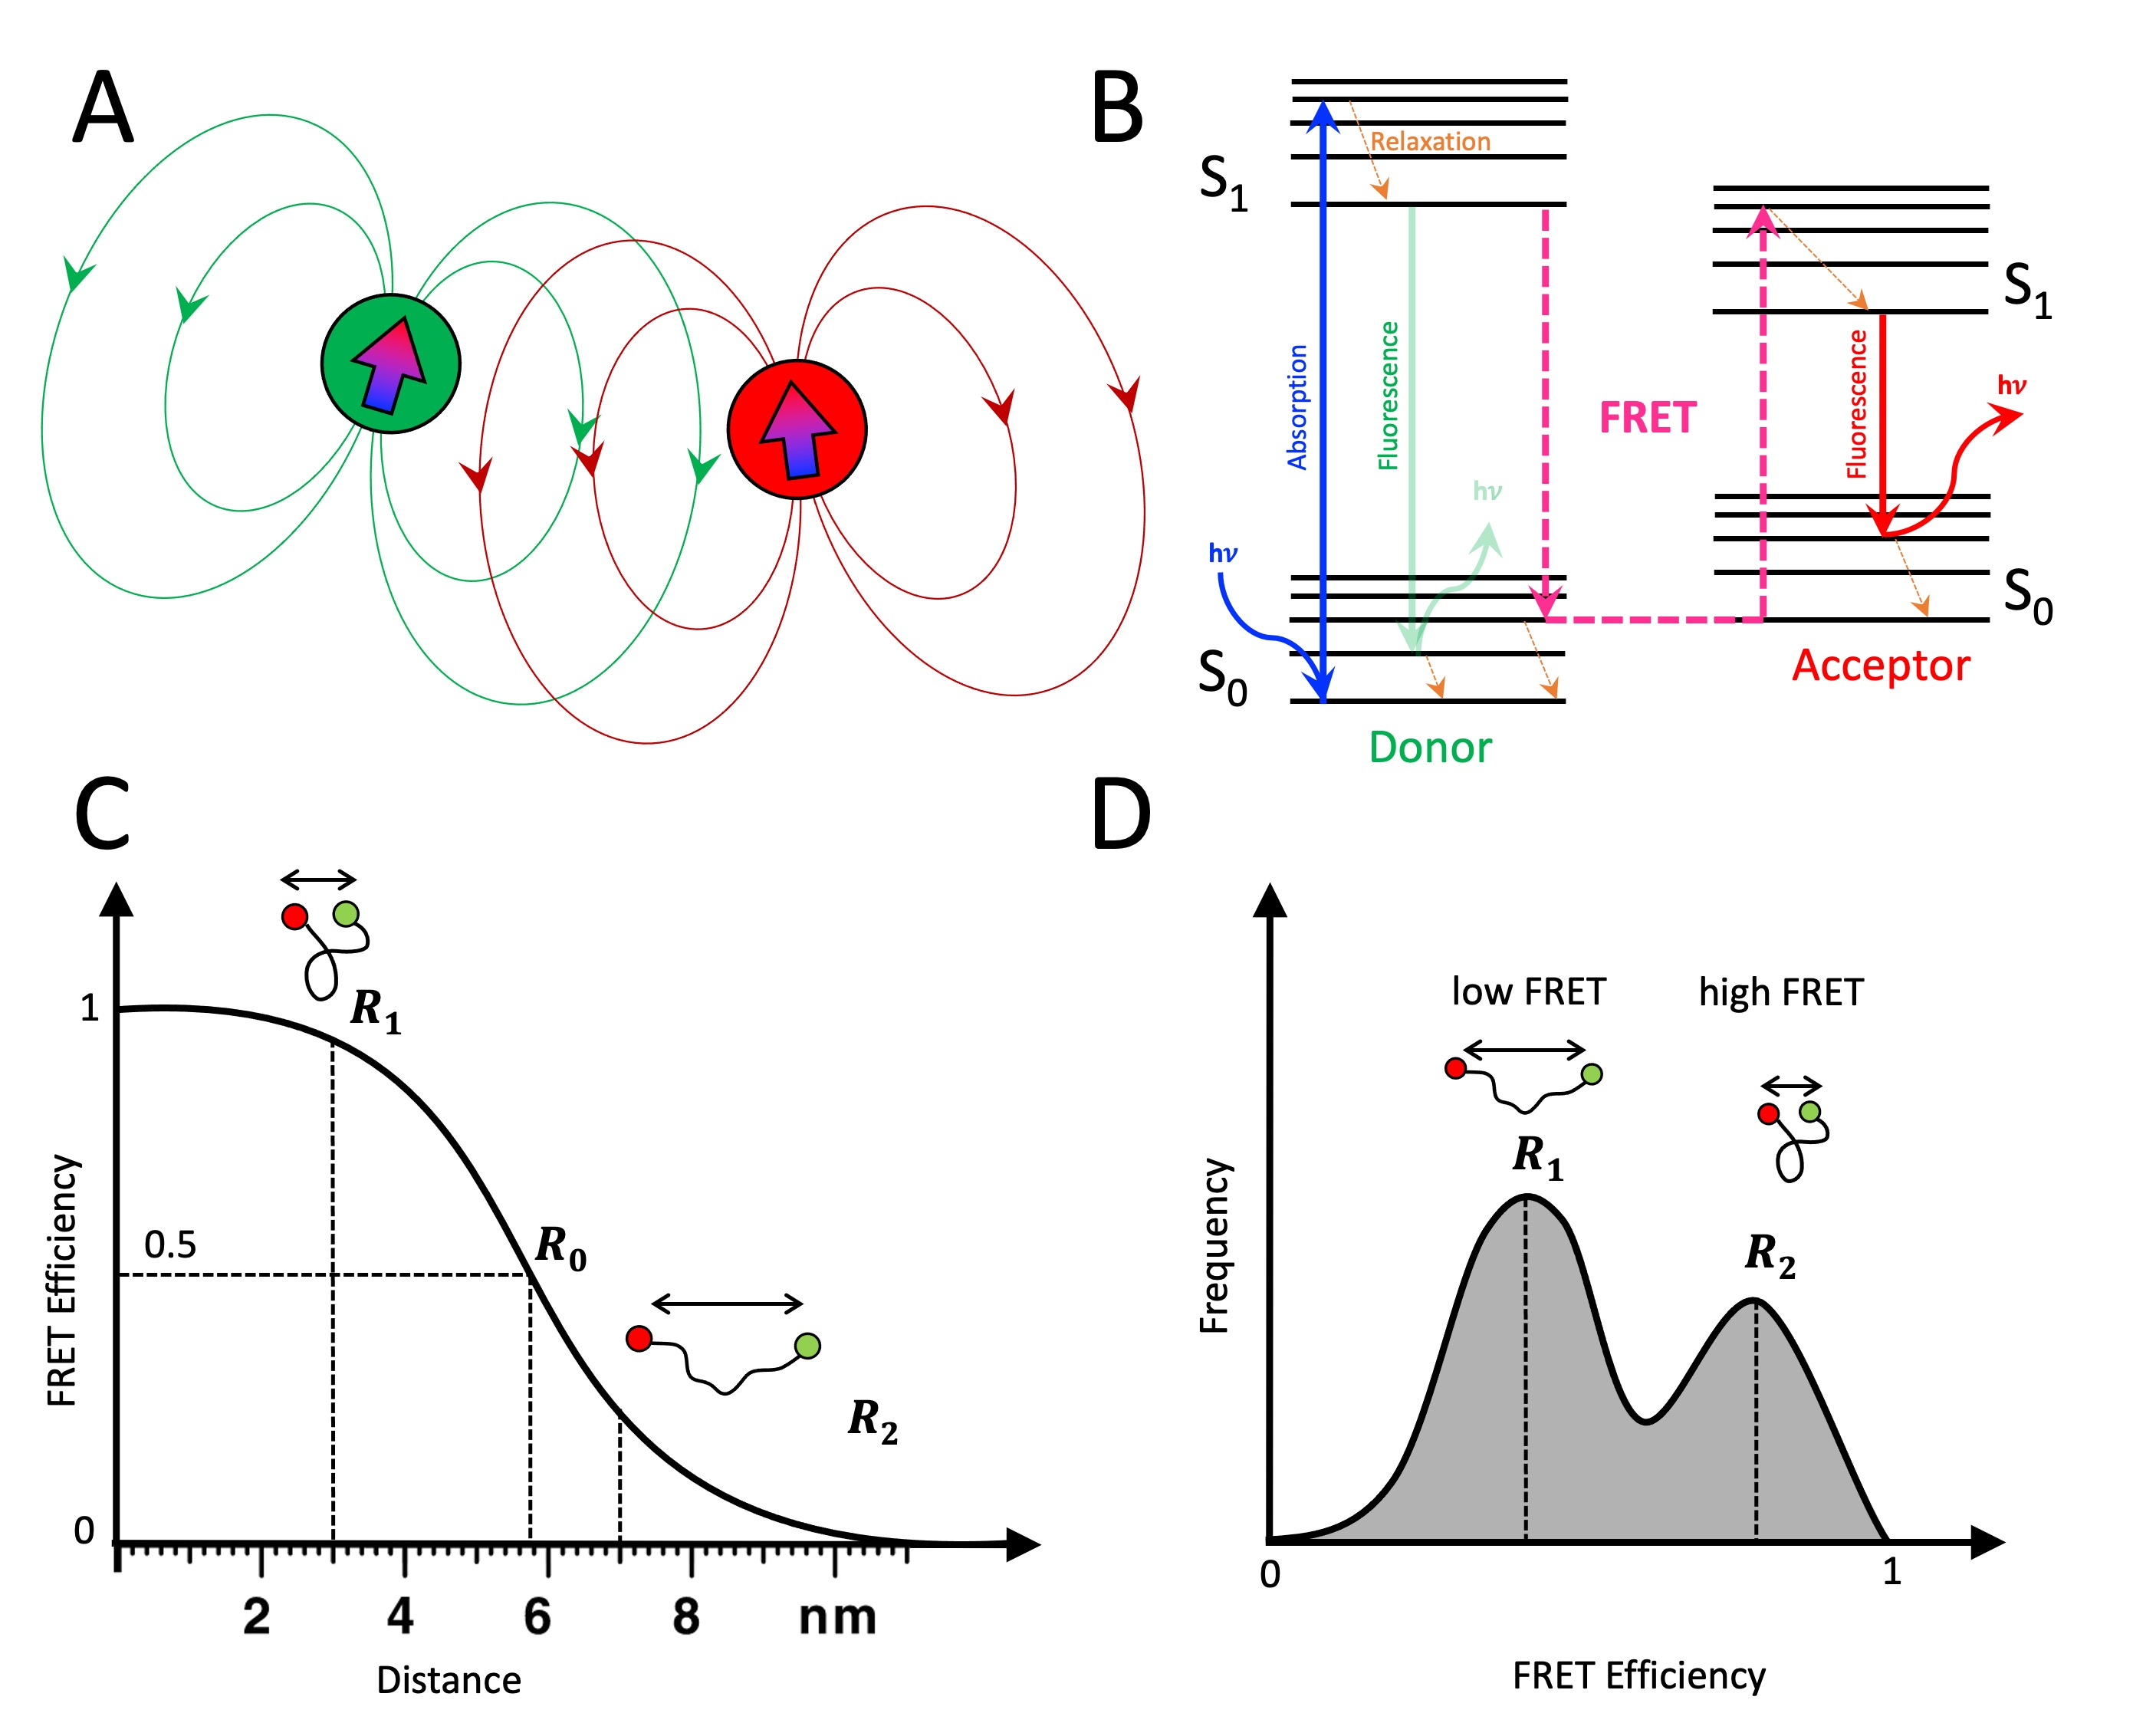
\includegraphics[width=\textwidth]{chapters/figures/FRET_concept.jpg}
    \caption{\label{fig:FRET_concept} 
    Fundamental concepts of FRET.
    A) Coulombic dipole-dipole interaction between representative donor and acceptor fluorophores (green and red circles, respectively).
    The polarity of the dipole moment is indicated by an arrow, where red indicates a positive charge and blue indicates a negative charge. 
    %%The electromagnetic field of the dipoles is shown for each molecule in green and red, and the colored arrows indicate the field polarity.
    B) Jablonski diagram of FRET. A fluorophore absorbs a photon of energy, $h\nu$, and an electron is promoted (blue arrow) from the ground state ($S_0$) to the excited state ($S_1$).
    In the absence of FRET, the electron relaxes to the ground state, emitting a photon (transparent green arrow). 
    If an acceptor fluorophore spectrally overlaps with the donor fluorophore is nearby, energy can be transferred non-radiatively to the acceptor fluorophore, where a ground state electron is promoted to the excited state (this process is undergone by a virtual photon, and is represented by the pink, dashed arrows). 
    Upon relaxation back to the ground state, a photon of lower energy is emitted from the acceptor. 
    Orange arrows indicate possible relaxation events to lower energy states. 
    C) FRET efficiency as a nanoscale \enquote{ruler}. 
    Efficiency of energy transfer is inversely proportional to the sixth power of the distance between the centers of the donor and acceptor molecules.
    The characteristic radius, $R_0$, occurs when the FRET efficiency $=0.5$.
    Two example molecules/conformations are shown, where $R_1 \approx 3$~nm and $R_2 \approx 7$~nm. 
    This relationship allows observation of small and precise changes in distances on the scale of 3-10 nm.
    D) Example FRET efficiency histogram with two distances, $R_1$ and $R_2$.
    A low FRET efficiency corresponds to a shorter distance between molecules and vice versa, i.e. $R_1 > R_2 \rightarrow E_1 < E_2$.}
\end{figure}

As discussed in Section~\ref{sec:FRET_intro}, FRET is driven by a Coulombic interaction between the transition dipole moments of a donor and acceptor fluorophore~(Fig.~\ref{fig:FRET_concept}A).
If the spectral overlap between these fluorophores is aligned, i.e. the absorbance band of the acceptor sufficiently overlaps with the excitation band of the donor, a resonance condition can be established. 
In this scenario, non-radiative energy transfer is possible from the excited donor fluorophore to the acceptor fluorophore~(Fig.~\ref{fig:FRET_concept}B). 
The efficiency of energy transfer decreases as $R^{-6}$ between the donor and acceptor molecules. 
Figure~\ref{fig:FRET_concept}C depicts the relationship between FRET efficiency and distance, i.e. a longer length ($R_2$) between fluorophores corresponds to a lower FRET efficiency, and a shorter distance ($R_1$) corresponds to a higher FRET efficiency.
Figure~\ref{fig:FRET_concept}D provides an example of FRET efficiency histograms for $R_1$ and $R_2$, where $R_1 > R_2$ and $E_1 < E_2$.

The FRET efficiency, $E$, can be calculated from $R$ when the fluorophores are approximated as point dipoles.
In other words, the size of the fluorophores must be much smaller than $R$ for accurate calculation of $E$. Formally, $E$ is defined as:

\begin{equation}
\label{eqn:E}
E=\frac{1}{1+(R/R_0)^6}
\end{equation}

\noindent
Where $R$ is the inter-dye distance and $R_0$ is the characteristic distance at which 50\% of the energy is transferred.
$R_0$ depends on four variable parameters: i) the orientation factor, $\kappa^2$, ii) the refractive index of the medium, $n$, iii) the quantum yield of the donor fluorophore, $\phi_D$, and iv) the spectral overlap term, $J(\lambda)$:

\begin{equation}
\label{eqn:R_0^6}
R_0^6 = \frac{9ln(10)}{128\pi^5 N_A} \frac{\kappa^2 \phi_D}{n^4}J(\lambda)
\end{equation}

\noindent
Where $N_A$ is Avogadro's number and $J(\lambda)$ is defined in terms of the donor fluorescence, $f_D(\lambda)$:

\begin{equation}
\label{eqn:J}
J(\lambda) = \int f_D(\lambda)\epsilon_A(\lambda)\lambda^4 d\lambda
\end{equation}

\noindent
Where $\epsilon_A$ is the molar extinction coefficient of the acceptor.
Here, we can see that $E$ is affected by the degree of spectral overlap between the donor emission and acceptor absorption spectra. 

Notably, the changing parameters ($R$, $\kappa^2$, $n$, $\phi_D$) complicate the calculation of distance measurements.
For example, $\kappa^2$ is often taken to be $\frac{2}{3}$.
However, $\kappa^2$ ranges between $1 - 4$.
The assumption that $\kappa^2 = \frac{2}{3}$ can be applied when the isotropic orientations of the donor and acceptor dipole moments are randomized and reorienting rapidly across the lifetime of the excited state of the donor in the presence of an acceptor~\cite{van_der_meer_2013}. 
In addition, photophysical properties such as quantum yields, spectral overlap, and bleaching also complicate FRET calculations. 
Thus, careful control measurements and the application of correction factors~\cite{lee_BPJ_2005, ingargiola_BioRxiv_2017} are required for accurate distance calculations using FRET theory.
A detailed explanation of the FRET correction factors is available in Section~\ref{sec:E_apdx} and Section~\ref{sec:correction_factors}.

\section{Single molecule studies
\label{sec:sm_intro}}

\begin{figure}
    \centering
    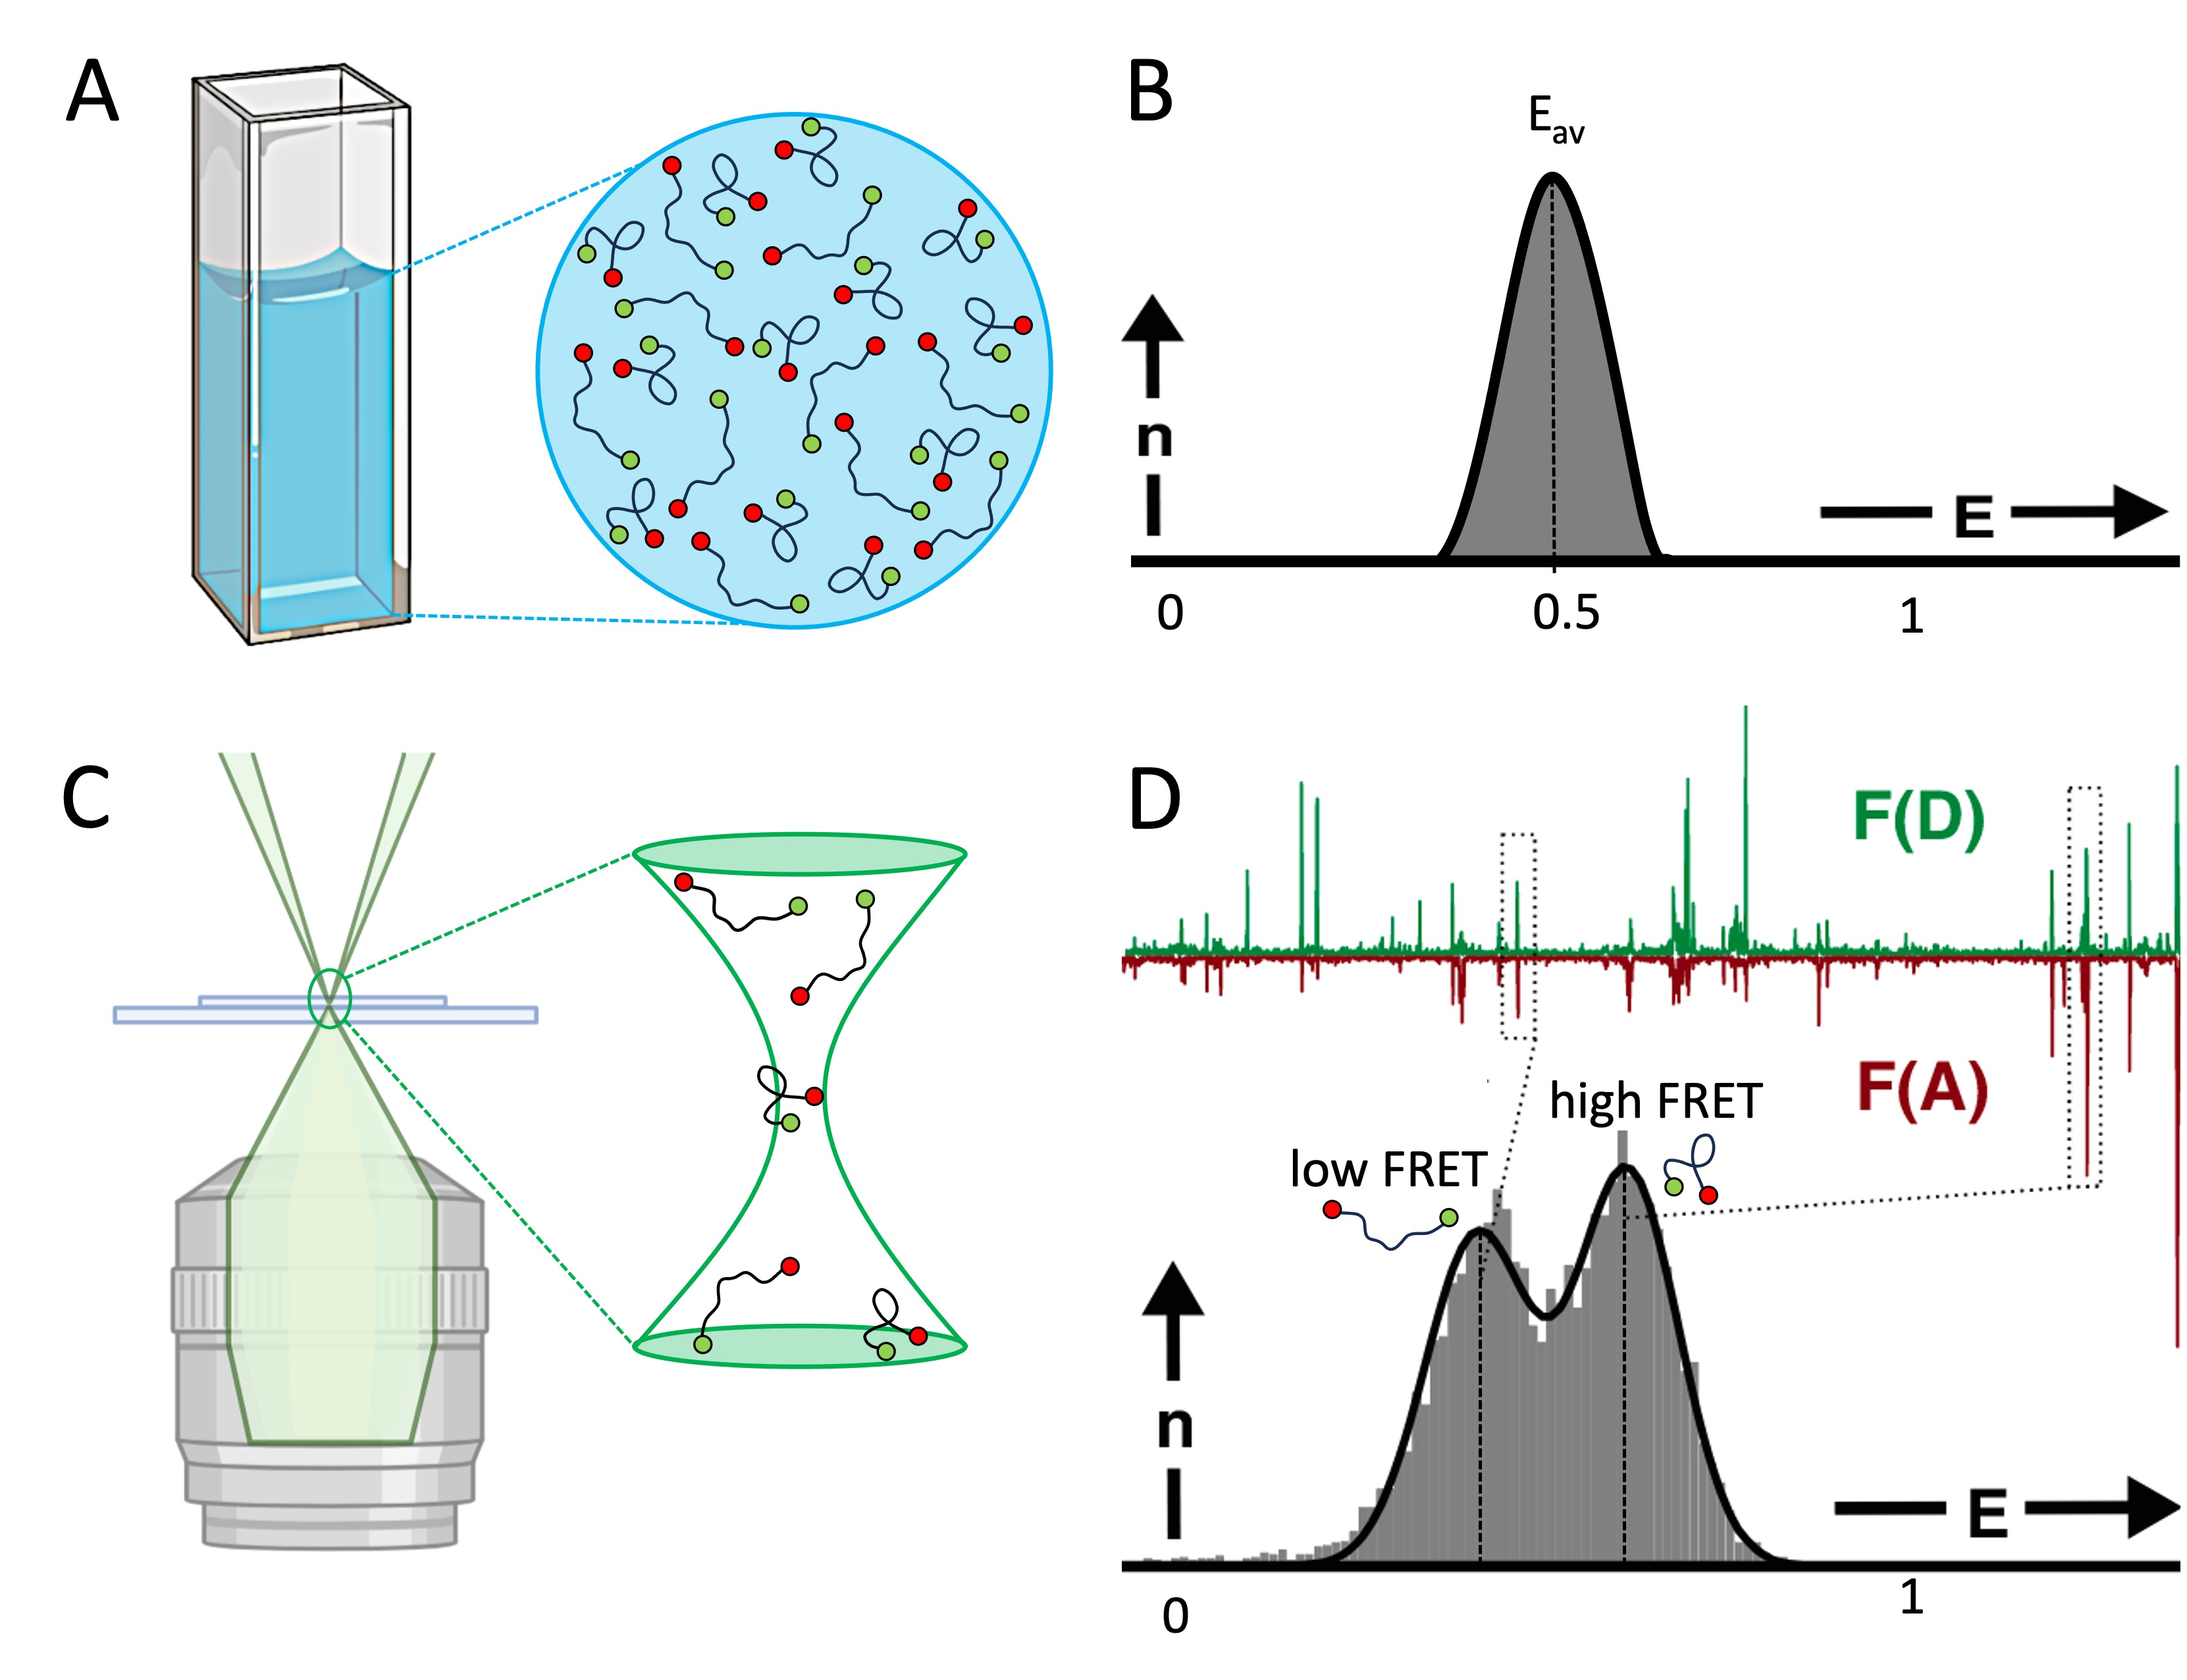
\includegraphics[width=\textwidth]{chapters/figures/smFRET_vs_ensemble.jpg}
    \caption{\label{fig:smFRET_vs_ensemble} 
    Ensemble FRET vs. single molecule FRET (\ac{smFRET}) studies of a representative doubly-labeled molecule.
    A) Example bulk FRET experiment. 
    An example of a typical ensemble study where the FRET efficiency of a high concentration sample of a flexible molecule labeled with a donor and acceptor fluorophore on each end is measured.
    B) Results of the bulk FRET experiment.
    The histogram illustrates the average FRET efficiency, $E_{av}$, measured in a bulk FRET experiment. 
    C) Example smFRET experiment.
    A confocal microscope is used to measure the FRET efficiency of one molecule ($\leq 100$~pM) at a time as it passes through the $1$~fL confocal volume.
    D) Time trace of smFRET measurement and resulting FRET efficiency histogram.
    Top: smFRET time trace showing the fluorescent bursts of the doubly-labeled molecule as it crosses the confocal volume, where $F(D)$ (green) is the donor fluorescence signal and $F(A)$ (red) is the acceptor fluorescence signal.
    The boxed coincident bursts are FRET bursts associated with different FRET efficiencies corresponding to low and high FRET populations of the flexible doubly-labeled molecule.
    }
\end{figure}

Extending FRET to the single molecule regime~\cite{deniz_PNAS_1999} allows us to obtain information on the sample heterogeneity that would otherwise be lost in ensemble measurements. 
Ensemble studies involve the simultaneous measurement of multiple molecules, with the goal of capturing an averaged signal.
Figure~\ref{fig:smFRET_vs_ensemble}A presents an example ensemble measurement where a flexible molecule, say single-stranded DNA, is labeled at both ends with a donor and acceptor dye.
The molecule in question may sample many conformations which correspond to different FRET distances.
However, when measured in bulk the average FRET efficiency, $E_{av}$, is represented by a single, narrow peak (Fig.~\ref{fig:smFRET_vs_ensemble}B).

In contrast, single molecule studies aim to measure individual molecules one at a time as they traverse the confocal volume, which is approximately $1\mu m^3$ (Fig.~\ref{fig:smFRET_vs_ensemble}C).
Measurement of a one molecule at a time allows identification of sub-populations within a sample. 
Figure~\ref{fig:smFRET_vs_ensemble}D presents a single-molecule FRET (\ac{smFRET}) measurement of a molecule with two distinct FRET efficiencies, where the time trace of the fluorescent signals arising from the donor and acceptor molecules ($F(D)$ in green and $F(A)$ in red, respectively) is presented on top and the corresponding FRET efficiency histogram is presented on the bottom.
With this example in mind, it is clear that ensemble measurements, i.e. measurements taken at concentrations $> 100$~pM result in signal averaging and loss of information, especially in the case of biomolecules that have asynchronized moving parts.
The undeniable benefit of smFRET studies is that we can capture the FRET efficiencies of sub-populations corresponding to the different conformations, i.e. inter-dye distances, of a single molecule.
% add section reference

However, single molecule measurements must be carried out at concentrations $\leq 100$ pM.
This ensures that only one molecule is being measured at any given time.
As I will explain in greater detail in Chapter~\ref{chpt:ht-smFRET}, this requirement establishes smFRET as an inherently low-throughput technique.

\section{FRET spectroscopy
\label{sec:FRET_intro}}

FRET efficiency is typically determined experimentally via lifetime measurements or ratiometric intensity measurements.
Lifetime measurements require advanced electronics, such as used in \ac{TCSPC} setups.
In these experiments, the lifetime of the donor in presence of the acceptor is shortened with respect to the intrinsic lifetime of the donor, i.e. the lifetime of the donor in the absence of the acceptor.
The FRET efficiency is then defined as:

\begin{equation}
    \label{eqn: E_lifetime}
    E = 1 - \frac{\tau_{FRET}}{\tau_D}
\end{equation}

\noindent
where $\tau_{FRET}$ is the lifetime of the donor in the presence of an acceptor and $\tau_D$ is the intrinsic lifetime of the donor.

In contrast, ratiometric measurements are more accessible, as they do not require advanced hardware, as in the case of \ac{TCSPC}. 
In these experiments, the fluorescence intensities of the donor and acceptor, specifically $F_{D_{ex}D_{em}}$ and $F_{D_{ex}A_{em}}$, are used to calculate the FRET efficiency, or, more accurately, the proximity ratio, $E_{PR}$:

\begin{equation}
    \label{eqn: E_ratiometric}
    E_{PR}=\frac{F_{D_{ex}A_{em}}}{F_{D_{ex}A_{em}}+F_{D_{ex}D_{em}}}
\end{equation}

\noindent
Where $E_{PR}$ is the uncorrected FRET efficiency.

Due to systematic errors in the measurement of fluorescence intensities, $F_{D_{ex}D_{em}}$ and $F_{D_{ex}A_{em}}$, ratiometric calculation of $E$ requires three correction factors, $l$, $d$, and $\gamma$.

\begin{description}
    \item[$Lk$: Leakage] The \enquote{leakage} factor accounts for the presence of donor excitation detected in the acceptor channel.
    While the majority of leakage can be filtered out using the appropriate optical filters, a small percentage of contaminating signal would be falsely attributed to fluorescence arising from the acceptor. 
    \item[$Dir$: Direct Excitation] In order to assume that fluorescence arising from the acceptor molecule is solely due to FRET, we must apply a correction factor that accounts for direct excitation of the acceptor molecule by the donor laser.
    \item[$\gamma$: $\gamma$ Factor] The detection efficiency correction factor accounts for the different quantum yields of the fluorophores and the photon detection efficiencies of the detectors for the emission bands of the donor and acceptor fluorophores.
\end{description}

Equations for the $Lk$, $Dir$ are discussed in Section~\ref{sec:correction_factors}. 
A thorough discussion of the proximity ration, $E_{PR}$, and the $\gamma$-corrected $E$ is presented in Section~\ref{sec:E_apdx}.

\newpage

%%%%%%%%%%%%%%%%%%%%%%%%%%%%%%%%%%%%%%%%%%%%%%%%%%%%%%%%%%%%%%%%%%%
\section{Molecular sorting via ALEX}
\label{sec:ALEX_intro}

\begin{wrapfigure}{r}{0.5\textwidth}
    \centering
    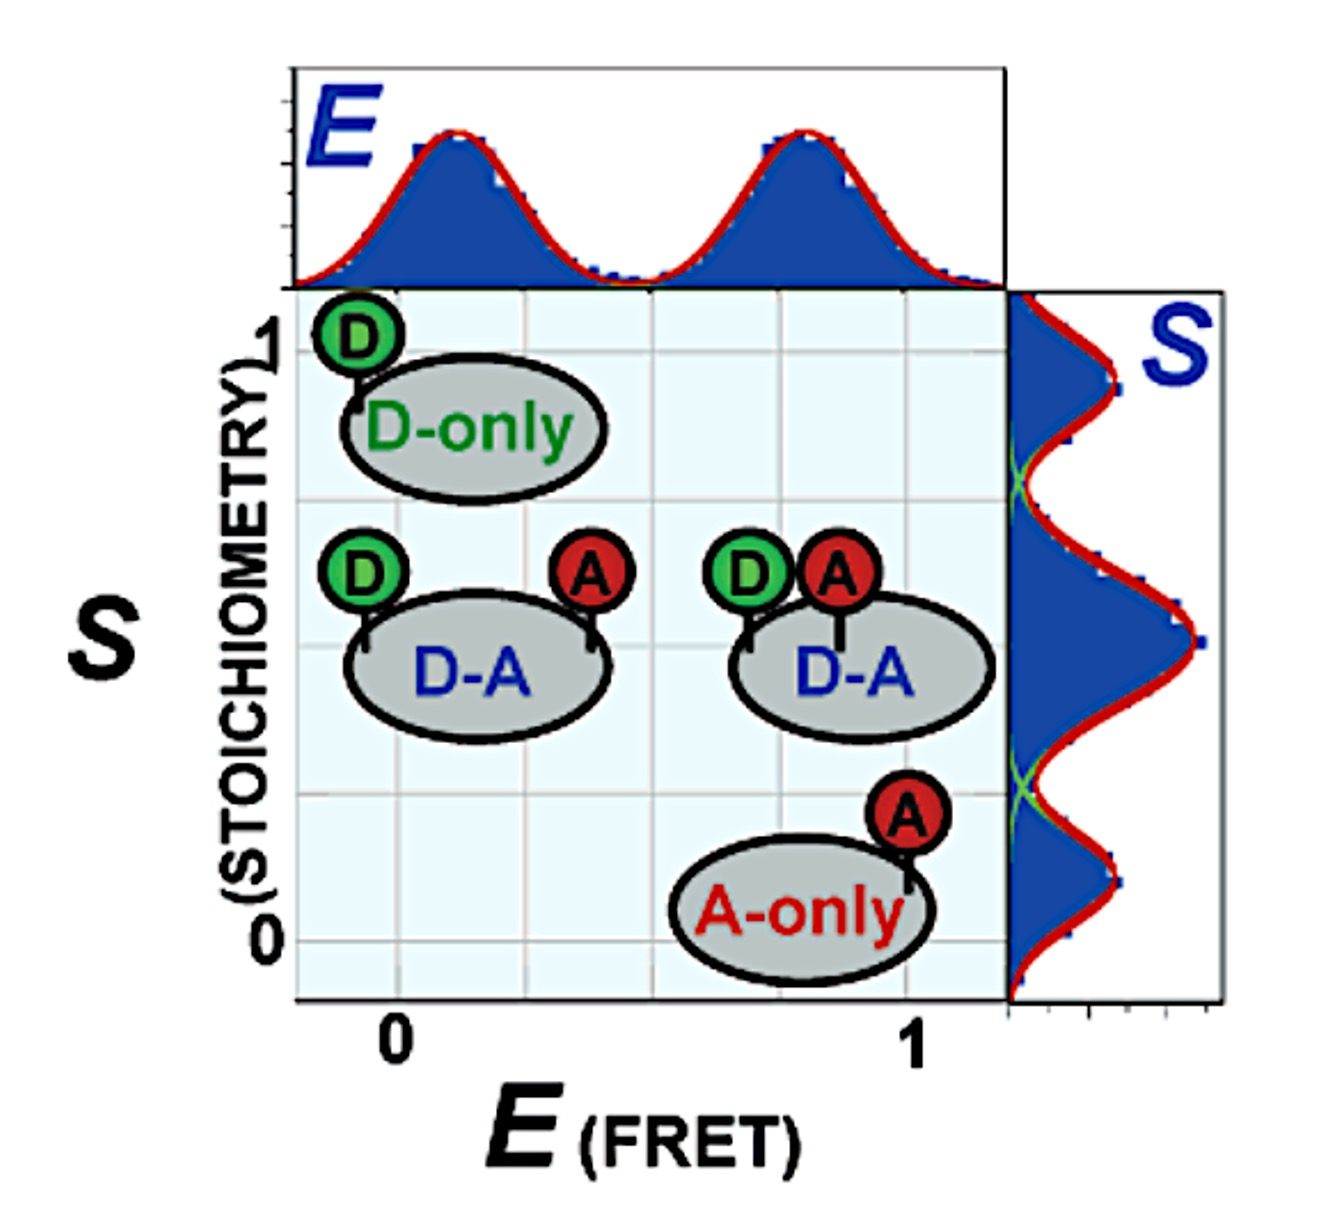
\includegraphics[width=0.48\textwidth]{chapters/figures/FAMS.jpg}
    \caption{\label{fig:FAMS} 
    \ac{FAMS} using  using  \ac{ALEX}.  
    2D $E - S$ histogram separates donor-only (D-only),  acceptor-only (A-only), and FRET (D-A) sup-populations.  
    In addition, FRET populations corresponding to different inter-dye distances may also be separated. 
    $E$ sorts species according to FRET efficiency, thereby reporting on inter-dye distance. 
    $S$ sorts on donor-acceptor stoichiometry,  reporting  on  interactions.  Sorting  is  also  possible  using  1D  histograms, where the red line indicates a sum  of fits and the green line indicates individual fits. 
    Figure adapted from Kapanidis \textit{et al}, 2005~\cite{kapanidis_ACR_2005}.
    }
\end{wrapfigure}

Single-laser excitation can be used in \ac{smFRET} experiments, however, it is unable to distinguish between singly-labeled donor-only molecules or doubly-labeled molecules with only one active acceptor dye from molecules with low FRET efficiency. 
This includes molecules in which the donor and acceptor inter-dye distance exceeds $R_0$. 
To address this limitation, alternative excitation methods such as \ac{ALEX} using two laser sources were developed~\cite{kapanidis_PNAS_2004}.

In \ac{ALEX}, two \ac{CW} lasers are rapidly alternated on a timescale of a few tens of microseconds. 
This timescale is shorter than the transit time of individual molecules through each excitation spot. 
This alternation scheme allows for the separation of doubly-labeled FRET species from singly-labeled donor- or acceptor-only molecules by calculating a simple uncorrected stoichiometry ratio, $S$, defined in section~\ref{sec:uncorrected_S_apdx}.

By combining the values of $E$ and $S$, both calculated from single-burst intensities in each channel during each excitation period, ALEX enables \enquote{digital sorting}, or \ac{FAMS}, of different burst populations in the $(E, S)$ plane.
Figure~\ref{fig:FAMS} presents a two-dimensional \enquote{ALEX histogram} where all bursts detected during a measurement can be represented and selected for further quantitative analyses~\cite{kapanidis_PNAS_2004,lee_BPJ_2005,laurence_PNAS_2005,muller_BJ_2005} (reviewed in Kapanidis \textit{et al.}, 2005~\cite{kapanidis_ACR_2005}).
Thus, introduction of a second laser in \ac{ALEX} effectively extends the number of sub-populations that can be separated. 

More recently, \ac{ALEX} has been extended to pulsed laser excitation schemes, such as \ac{nsALEX} or \ac{PIE}~\cite{laurence_PNAS_2005, muller_BJ_2005}. 
\ac{ALEX} has also been extended to multiple laser excitations, allowing even more powerful molecular sorting applications~\cite{lee_BPJ_2007, yim_CC_2012}.

%%%%%%%%%%%%%%%%%%%%%%%%%%%%%%%%%%%%%%%%%%%%%%%%%%%%%%%%%%%%%%%%%%
\section{Periodic Acceptor Excitation}
\label{sec:PAX_intro}

\begin{figure}
    \centering
    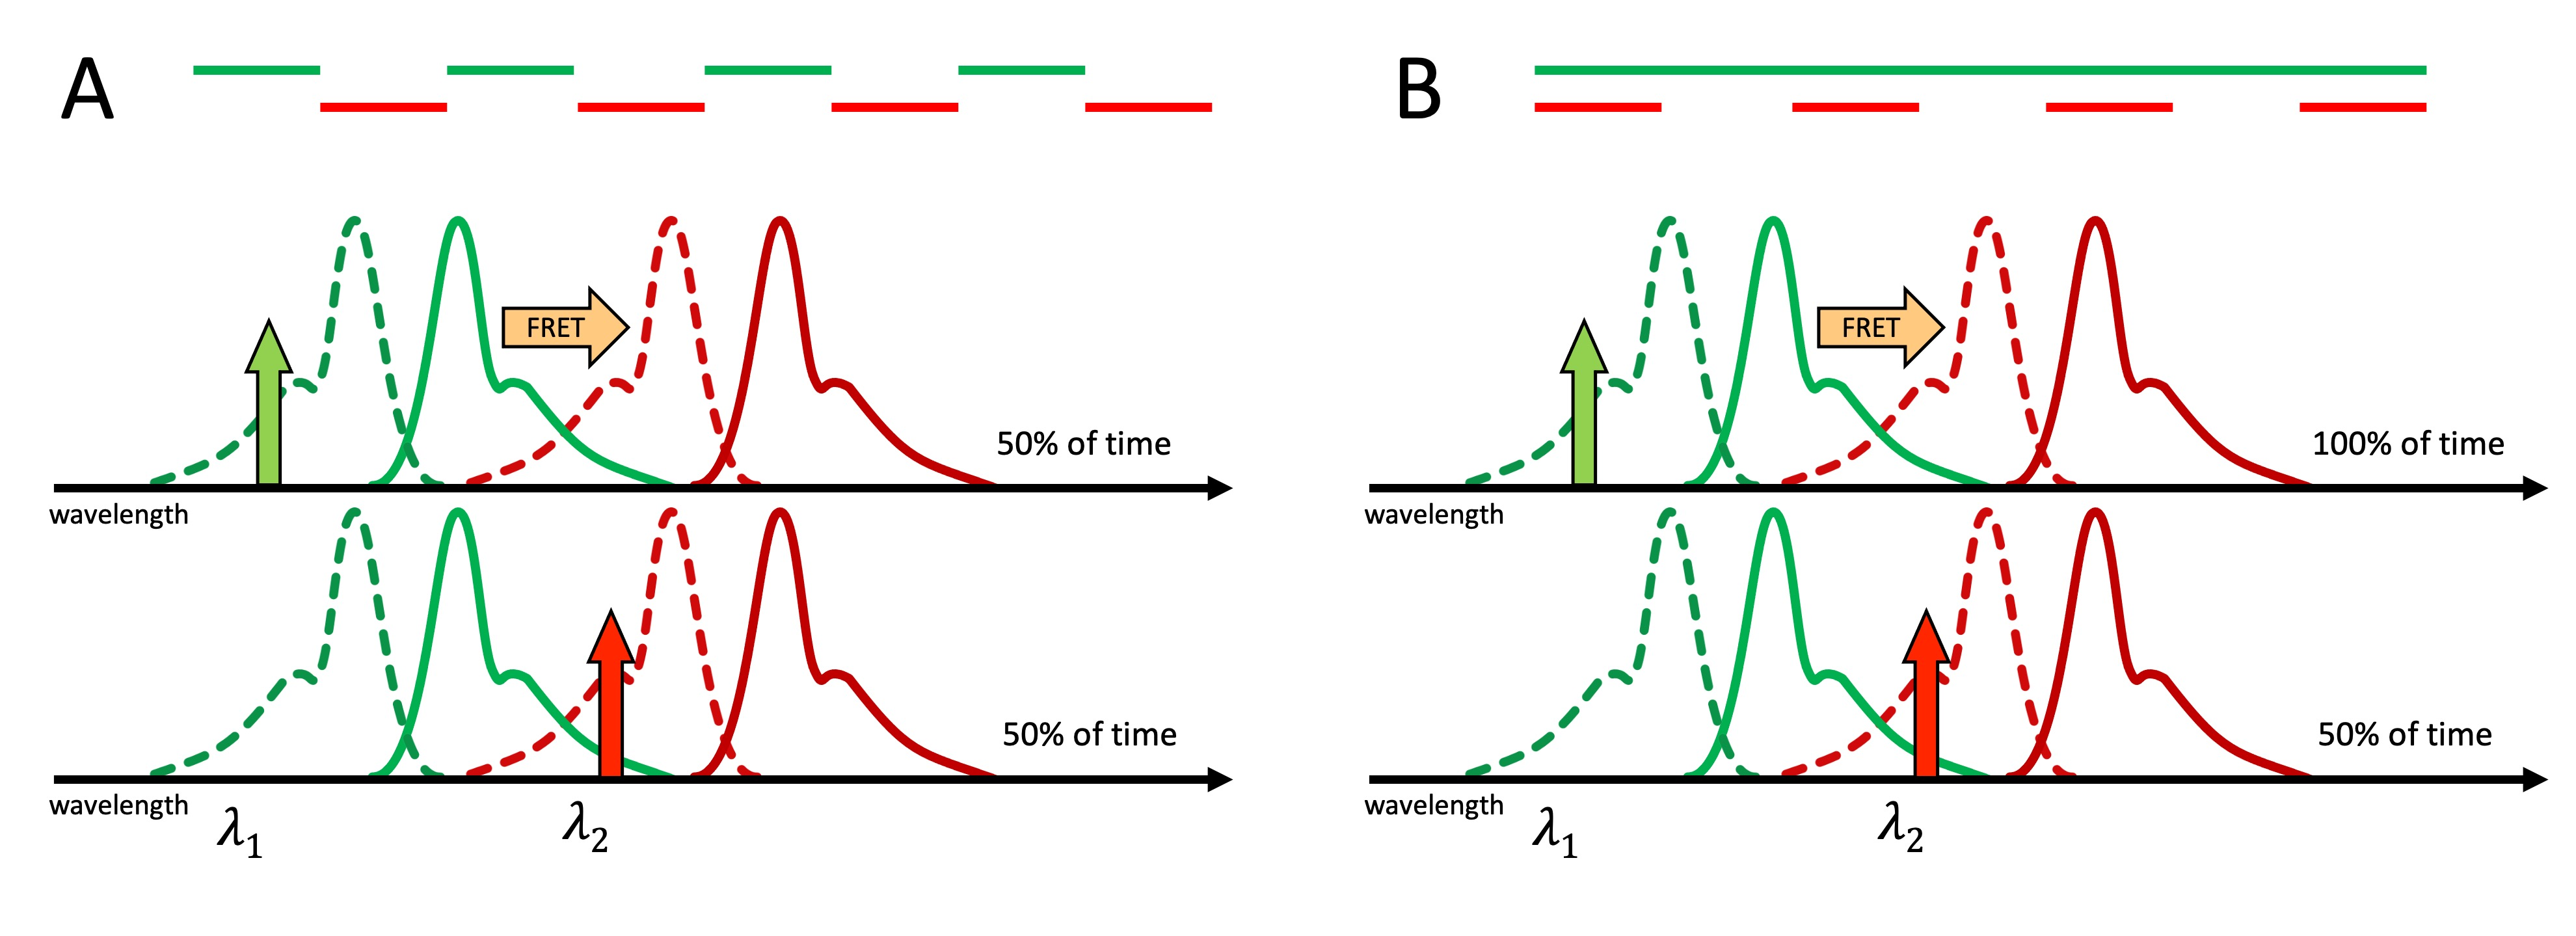
\includegraphics[width=\textwidth]{chapters/figures/ALEX_vs_PAX.jpg}
    \caption{\label{fig:ALEX_vs_PAX} 
    Comparison of \ac{ALEX} and \ac{PAX} techniques in \ac{smFRET}.
    A) Top: in the context of \ac{ALEX}, both lasers are alternated such that each excitation period only has one laser excitation.
    Bottom: absorption and emission spectra of the donor (green) and acceptor (red) fluorophores are depicted, where dashed line indicate absorbance and solid lines indicate emission. 
    Laser excitation wavelengths, $\lambda_1$ represents the donor excitation wavelength, $\lambda_1$ represents the acceptor excitation wavelength. 
    B) Top: in the context of \ac{PAX}, excitation by the green laser is continuous while only the acceptor excitation is alternated.
    In both cases, FRET occurs during the donor excitation period.
    However, in \ac{ALEX} this is limited to half the time, while in \ac{PAX} FRET can occur during both excitation periods. 
    }
\end{figure}

\ac{PAX} is a variant of the dual-excitation alternation scheme used in \ac{ALEX}, (Fig.~\ref{fig:ALEX_vs_PAX}A). 
However, \ac{PAX} is a simplified implementation of \ac{ALEX} in which only the acceptor excitation is modulated (Fig.~\ref{fig:ALEX_vs_PAX}B). 
This modification preserves molecular sorting capabilities while simplifying the experimental setup~\cite{doose_EBJ_2007}.
Specifically, it is cheaper and easier to implement as only one laser is alternated, while in \ac{ALEX} two modulators, one for each laser, are required.

In smFRET-PAX, an \ac{AOM} is used to alternate the red laser only. 
The primary advantage of \ac{PAX} over \ac{ALEX} is simplified alignment, as only the red laser is diverted into the \ac{AOM}. However, one disadvantage of \ac{PAX} is the potential for additional photobleaching of fluorescent dyes due to the higher acceptor excitation power used to compensate for the lower detection efficiency in the red part of the spectrum. 
Further studies are needed to fully quantify this photobleaching effect.

